\documentclass[10pt,final,leqno]{beamer}

%\usetheme{CambridgeUS}
\usetheme[style=ntnu,language=en]{ntnu2015}
%\usecolortheme{orchid}

\usepackage[utf8]{inputenc}
\usepackage[T1]{fontenc}

% Paths
\newcommand{\figs}{../figs}
\newcommand{\data}{../data}
\newcommand{\code}{../code}

% URL styles
\usepackage{url}
\urlstyle{sf}

% Units
\usepackage[detect-weight=true, binary-units=true]{siunitx}
\DeclareSIUnit\flop{FLOPS}

% Math
\usepackage{amsmath}
\usepackage{amssymb}
\usepackage{bm}
\usepackage{nicefrac}
\newcommand{\dif}[1]{{\;\text{d}#1}}

% Graphics
\usepackage{graphicx}
\usepackage{caption}
%\usepackage{subcaption}
\graphicspath{{../figs/}}

% Tikz
\usepackage{tikz}
\usetikzlibrary{positioning,shapes,arrows,calc,intersections}
\usepackage{pgfplots}
\usepgfplotslibrary{dateplot}
\pgfplotsset{compat=1.14} 

% Colors
\definecolor{darkblue}{HTML}{00688B}
\definecolor{darkgreen}{HTML}{6E8B3D}
\definecolor{cadet}{HTML}{DAE1FF}
\definecolor{salmon}{HTML}{FFB08A}

\usepackage{algorithm}

% Listings
\usepackage{textcomp}
\usepackage{listings}
\lstset{
  keywordstyle=\bfseries\color{orange},
  stringstyle=\color{darkblue!80},
  commentstyle=\color{darkblue!80},
  showstringspaces=false,
  basicstyle=\ttfamily,
  upquote=true,
}
\lstdefinestyle{fortran}{
  language=Fortran,
  morekeywords={for},
  deletekeywords={status},
}
\lstdefinestyle{c}{
  language=C,
  morekeywords={include},
}
\lstdefinestyle{glsl}{
  language=C,
  morekeywords={attribute, vec2, vec3, vec4, varying, uniform, mat2, mat3, mat4},
}
\lstdefinestyle{cuda}{
  language=C,
  morekeywords={__global__, __device__, __host__, __shared__},
}
\lstdefinestyle{shell}{
  language=bash,
  morekeywords={mkdir, ssh, cmake},
}

% Double hlines
\usepackage{hhline}

% Misc
\usepackage{nth}

\subtitle{TMA4280---Introduction to Supercomputing}

\graphicspath {{../figs/}}

\AtBeginSection[]
{
 \begin{frame}<beamer>
 \frametitle{Outline}
 \tableofcontents[currentsection]
 \end{frame}
}

\begin{document}


\title{Discussion on Direct Solvers}
\institute{NTNU, IMF}
\date{February 27. 2017}
\author{Based on 2016v slides by Eivind Fonn}
%\author{Aurélien Larcher}


\maketitle

\begin{frame}
  \frametitle{The problem}
  \begin{itemize}
  \item We want to solve
    \[
      \bm A \bm x = \bm b, \qquad
      \bm b, \bm x \in \mathbb{R}^N, \qquad
      \bm A \in \mathbb{R}^{N \times N}
    \]
    where $\bm A$ is the system resulting from discretiziing a Poisson problem
    using finite differences (see the previous slides).
  \item We use standard notation for matrices and vectors, i.e.
    \[
      \begin{pmatrix}
        a_{1,1} & a_{1,2} & \cdots & a_{1,N} \\
        a_{2,1} & a_{2,2} & \cdots & a_{2,N} \\
        \vdots  & \vdots  & \ddots & \vdots  \\
        a_{N,1} & a_{N,2} & \cdots & a_{N,N}
      \end{pmatrix}
      \begin{pmatrix} x_1 \\ x_2 \\ \vdots \\ x_N \end{pmatrix} =
      \begin{pmatrix} b_1 \\ b_2 \\ \vdots \\ b_N \end{pmatrix}
    \]
  \end{itemize}
\end{frame}

\begin{frame}
  \frametitle{Computer algorithms}
  \begin{itemize}
  \item We know that the solution is given by
    \[ \bm x = \bm A^{-1} \bm b. \]
  \item Explicitly forming the inverse $\bm A^{-1}$ is expensive, prone to
    round-off errors, and something we seldom do on computers.
  \item Exception: Very small and frequently re-used sub-problems that are known
    to be well conditioned.
  \item Matrix inversion has the same time complexity as matrix multiplication
    (typically $\mathcal{O}(n^3)$).
  \item Instead, we implement algorithms that solve a linear system given a
    specific right-hand-side vector.
  \item The structure and properties of the matrix $\bm A$ determine which
    algorithms we can use.
  \end{itemize}
\end{frame}

\begin{frame}
  \frametitle{Computer algorithms}
  \begin{itemize}
  \item For example: if $\bm A$ is known to be orthogonal, then
    \[ \bm x = \bm A^\intercal \bm b. \]
  \item Orthogonal matrices are the exception, and not the rule.
  \item We are more likely to find and exploit properties such as
    \begin{itemize}
    \item Symmetry
    \item Definiteness
    \item Sparsity
    \item Bandedness
    \end{itemize}
  \item We will now consider a number of different algorithms, their
    implementation and usability in a parallel context.
  \end{itemize}

\medskip
All the methods rely on intensive use of basic linear algebra operations which should be optmized for performance.
\end{frame}

\begin{frame}
  \frametitle{Complexity of operations}

\textbf{Dot Product:}
\[
\alpha = \sum_i \bm x_i \bm y_i
\]

\medskip
The reduction incurs a cost of $log2(N)$ for $N/2$ processors.

\bigskip
\textbf{Scalar-Vector Product:}
\[
\bm y_i = \alpha \bm x_i
\]

\medskip
The operation parallelizes completely and has a constant complexity using $N$ processors

\end{frame}

\begin{frame}
  \frametitle{Complexity of operations}

\textbf{Vector Addition}:
\[
\bm z_i = \bm x_i + \bm y_i
\]

\medskip
The operation parallelizes completely and has a constant complexity using $N$ processors.
Also note the provided operation $AXPY$: $\bm y_i = \alpha\bm x_i + \bm y_i$.


\bigskip
\textbf{Sum of N Vectors of size M:}
\[
\bm y_i = \sum_k \bm x_{k,i}
\]

\medskip
The operation is a reduction for eah component and each component can be done in parallel. complexity is $log2(N)$ on $M N/2$ processors

\bigskip
\textbf{Sum of N Matrices of $\mathbb R^{M\times M}$:} Simple extension of the vector case.

\end{frame}


\begin{frame}
  \frametitle{Complexity of operations}

\textbf{Matrix-Vector Multiplication in $\mathbb R^{M\times N}$}:
\[
\bm y_i = \bm A_{ij} \; \bm x_j
\]

\medskip
The operation can be seem as $M$ inner-products of size $N$.
Two options are available depending on the loop ordering:
\begin{enumerate}
\item $i,j$: innner-product model
\item $j,i$: linear combination of column vectors
\end{enumerate}


\bigskip
The use of one or the other depends on the data layout of 2d arrays:
\begin{enumerate}
\item row-major: storage row by row (C/C++)
\item column-major: storage column by column (FORTRAN)
\end{enumerate}

\medskip
Complexity is bound to the reduction $log2(N)$ for $M N/2$ processors.

\medskip
For $M$ processors it is $O(N)$, ror $1$ processor it is $O(MN)$ 

\end{frame}

\begin{frame}
  \frametitle{Complexity of operations}

\textbf{Matrix-matrix Multiplication in $\mathbb R^{M\times N}$, $\mathbb R^{N\times L}$}:
\[
\bm A_{ij} = \bm B_{ik} \; \bm C_{kj}
\]

\medskip
Six options are available depending on the loop ordering $i,j,k$.

\medskip
Complexity is bound to the reduction $log2(N)$ for $M N L/2$ processors.


\medskip
For square matrices: $N^3$ processors it is $O(log2(N))$, for $N^2$ processor it is $O(N)$, and for $N$ processor it is $O(N^2)$

\end{frame}

%------------------------------------------------------------------------------
\begin{frame}
  \frametitle{Linear algebra packages}

\begin{tabular}{l|l}
\href{http://www.netlib.org/blas/}{BLAS} & Linear algebra routines, reference (FORTRAN)\\
\href{http://www.openblas.net/}{OpenBLAS} & Optimized multithreaded BLAS (C, Assembly)\\
\href{http://www.netlib.org/lapack/}{LAPACK} & Direct and eigenvalue solvers (FORTRAN)\\
\href{http://arma.sourceforge.net/}{Armadillo} &  Linear algebra package (C++)\\
\href{http://faculty.cse.tamu.edu/davis/suitesparse.html}{SuiteSparse} &  Factorizations with GPU support\\
\href{http://mumps.enseeiht.fr/}{MUMPS} & Parallel sparse matrix direct solvers (FORTRAN)\\
\end{tabular}

\bigskip
Software packages like PETSc, Trilinos provde general interfaces to these packages.

\end{frame}

%------------------------------------------------------------------------------

\begin{frame}
  \frametitle{Linear algebra performance}

Performance is measured with the number of floating-point operations per second (FLOPS).

\medskip
Performance of linear algebra operations is heavily influenced by:
\begin{enumerate}
\item ratio between computations and data movement, 
\item memory access patterns.
\end{enumerate}

\medskip
Performance can be further improved by parallelism: some algorithms offer intrisically more opportunities for parallelism than other (think in terms of data dependencies)

\end{frame}

%------------------------------------------------------------------------------

\begin{frame}
  \frametitle{Linear algebra performance}

Vector-vector operations (AXPY):
\begin{enumerate}
\item $2n$ ops
\item $2n$ data
\end{enumerate}
$\rightarrow$ $r_{ops/data} = O(1)$ performance guided by ILP and caching limits.

\bigskip
Matrix-matrix operations (MM): $A \in \mathbb R^{mxk}, B \in \mathbb R^{kxn}$
\begin{enumerate}
\item $mn(2k-1)$ ops
\item $(m+n)k$ data
\end{enumerate}
$\rightarrow$ $r_{ops/data} = O(N)$ data reuse by several floating-point operations. 

\medskip
Such considerations were explained when introducing computational efficiency of dense linear algebra benchmarks (LINPACK) vs. sparse matrix benchmarks (HPCG)

\end{frame}

%------------------------------------------------------------------------------

\begin{frame}
  \frametitle{BLAS}
  \begin{itemize}
  \item A very helpful library here is \emph{BLAS}: Basic Linear Algebra
    Subprograms.
  \item BLAS is an old specification from the late seventies and early eighties.
  \item It consist of a collection of functions with strangely cryptic and short
    names.
  \item Can be installed on Ubuntu with
    \texttt{sudo apt-get install libblas-dev}.
  \item On Vilje, Intel's implementation of BLAS is available under \emph{MKL}:
    the Math Kernel Library, and on Lille OpenBLAS is available.
  \end{itemize}
\end{frame}


\begin{frame}
  \frametitle{BLAS levels}
  \begin{itemize}
  \item BLAS functions are organized by \emph{level}.
  \item Level 1: vector-vector operations.
    \[ \bm y = \alpha \bm x + \bm y \]
    \texttt{daxpy(n, alpha, y, 1, x, 1)}
  \item Level 2: matrix-vector operations.
    \[ \bm y = \alpha \bm A \bm x + \beta \bm y \]
    \texttt{dgemv('N', m, n, alpha, A, m, x, 1, beta, y, 1)}
  \item Level 3: matrix-matrix operations
    \[ \bm C = \alpha \bm A \bm B + \beta \bm C \]
    \texttt{dgemm('N', 'N', m, n, k, alpha, A, m, B, k, C, m)}
  \end{itemize}
\end{frame}

\begin{frame}
  \frametitle{BLAS conventions}
  \begin{itemize}
  \item All functions in BLAS starts with one of the letters
    \begin{itemize}
    \item[s] for \emph{single}.
    \item[d] for \emph{double}.
    \item[c] for \emph{single complex}.
    \item[z] for \emph{double complex}.
    \end{itemize}
  \item If the operation involves a matrix, two letters describing the matrix
    format follow. The most important of these are
    \begin{itemize}
    \item[ge] for \emph{general} matrices.
    \item[po] for \emph{symmetric} matrices.
    \item[gb] for \emph{general banded} matrices.
    \item[pb] for \emph{symmetric banded} matrices.
    \end{itemize}
  \end{itemize}
\end{frame}

\begin{frame}
  \frametitle{BLAS}
  \begin{itemize}
  \item The BLAS home page can be found at http://netlib.org/blas/
  \item BLAS is written in Fortran and therefore expects Fortran memory layout
    (column-major ordering).
  \item For C, the \emph{CBLAS} implementation is popular. CBLAS supports both
    row- and column-major orders.
  \end{itemize}
\end{frame}

\begin{frame}[fragile]
  \frametitle{Serial BLAS}
\begin{lstlisting}[style=c, basicstyle=\ttfamily\footnotesize]
void MxV(double *u, double *A, double *v, int N)
{
  dgemv('N', N, N, 1.0, A, N, v, 1, 0.0, u, 1);
}

double innerproduct(double *u, double *v, int N)
{
  // Necessary adjustments must be made for MPI
  return ddot(N, u, 1, v, 1);
}
\end{lstlisting}
\end{frame}


\begin{frame}
  \frametitle{Simple example}
  Computing
  \[
    \alpha = \sum_{i=1}^K \bm v_i^\intercal \bm A \bm v_i
  \]
  where $\bm v \in \mathbb{R}^{N \times K}$ and
  $\bm A \in \mathbb{R}^{N \times N}$. There are $K$ terms, each of which
  require us to compute a matrix-vector product and an inner product.
\end{frame}

\begin{frame}[fragile]
  \frametitle{Serial}
\begin{lstlisting}[style=c, basicstyle=\ttfamily\footnotesize]
void MxV(double *u, double **A, double *v, int N)
{
  for (size_t i = 0; i < N; i++) {
    u[i] = 0.0;
    for (size_t j = 0; j < N; j++)
      u[i] += A[i][j] * v[j];
  }
}

double innerproduct(double *u, double *v, int N)
{
  double result = 0.0;
  for (size_t i = 0; i < N; i++)
    result += u[i] * v[i];
  return result;
}
\end{lstlisting}
\end{frame}

\begin{frame}[fragile]
  \frametitle{Serial}
\begin{lstlisting}[style=c]
double dosum(double **A, double **v, int K, int N)
{
  double alpha = 0.0, temp[N];
  for (size_t i = 0; i < K; i++) {
    MxV(temp, A, v[i], N);
    alpha += innerproduct(temp, v[i], N);
  }

  return alpha;
}
\end{lstlisting}
\end{frame}

\begin{frame}
  \frametitle{OpenMP micro-version}
  \begin{itemize}
  \item It is tempting to exploit all parallelism in sight. However, don't do
    that.
  \item Let us use OpenMP for micro-parallelism. That is, we exploit parallelism
    within the inner product and the matrix-vector operation.
  \item That means two fork/join operations per term, so $2K$ in total.
  \end{itemize}
\end{frame}

\begin{frame}[fragile]
  \frametitle{OpenMP micro-version}
\begin{lstlisting}[style=c]
void MxV(double *u, double **A, double *v, int N)
{
  #pragma omp parallel for schedule(static)
  for (size_t i = 0; i < N; i++) {
    u[i] = 0.0;
    for (size_t j = 0; j < N; j++)
      u[i] += A[i][j] * v[j];
  }
}
\end{lstlisting}
\end{frame}

\begin{frame}[fragile]
  \frametitle{OpenMP micro-version}
\begin{lstlisting}[style=c]
double innerproduct(double *u, double *v, int N)
{
  double result = 0.0;
  #pragma omp parallel for schedule(static) \
          reduction(+:result)
  for (size_t i = 0; i < N; i++)
    result += u[i] * v[i];
  return result;
}
\end{lstlisting}
\end{frame}

\begin{frame}
  \frametitle{OpenMP macro-version}
  \begin{itemize}
  \item The alternative is to exploit the coarsest parallelism: each iteration
    in the \texttt{dosum} method.
  \item In this case we perform exactly one fork and one join.
  \item Problem: the \texttt{dosum} method uses a temporary buffer for the
    matrix-vector multiplication, which cannot be shared between threads. We
    have to use a separate buffer for each thread.
  \end{itemize}
\end{frame}

\begin{frame}[fragile]
  \frametitle{OpenMP macro-version}
\begin{lstlisting}[style=c]
double dosum(double **A, double **v, int K, int N)
{
  double alpha = 0.0;
  double **temp = createMatrix(K, N);
  #pragma omp parallel for schedule(static) \
          reduction(+:alpha)
  for (size_t i = 0; i < K; i++) {
    MxV(temp[i], A, v[i], N);
    alpha += innerproduct(temp[i], v[i], N);
  }

  return alpha;
}
\end{lstlisting}
\end{frame}

\begin{frame}[fragile]
  \frametitle{MPI macro-version}
\begin{lstlisting}[style=c]
double dosumMPI(double **A, double **v,
                int myK, int N)
{
  double myalpha = dosum(A, V, myK, N);
  double alpha;
  MPI_Allreduce(&myalpha, &alpha, 1, MPI_DOUBLE,
                MPI_SUM, MPI_COMM_WORLD);
  return alpha;
}
\end{lstlisting}
  In addition to the usual MPI code, you have to decide on a particular division
  of the work among the nodes. For brevity's sake, it is left out in this
  example.
\end{frame}

\begin{frame}
  \frametitle{Speedup results}
  \begin{center}
    \begin{table}
      \caption{$N=2048$, $K=1024$}
      \bgroup\def\arraystretch{1.2}
      \begin{tabular}{rrrr}
        \hline
        Threads & Micro & Macro & MPI \\
        \hhline{====}
        1 & 1.00 & 1.00 & 1.00 \\
        2 & 1.84 & 1.83 & 1.56 \\
        4 & 2.79 & 2.76 & 3.46 \\
        \hline
      \end{tabular}
      \egroup
    \end{table}
    \begin{table}
      \caption{$N=16$, $K=32768$}
      \bgroup\def\arraystretch{1.2}
      \begin{tabular}{rrrr}
        \hline
        Threads & Micro & Macro & MPI \\
        \hhline{====}
        1 & 1.00 & 1.00 & 1.00 \\
        2 & 0.50 & 2.00 & 2.00 \\
        4 & 0.33 & 3.49 & 4.00 \\
        \hline
      \end{tabular}
      \egroup
    \end{table}
  \end{center}
\end{frame}

\begin{frame}
  \frametitle{Timing results}
  \begin{center}
    \begin{table}
      \caption{$N=2048$, $K=1024$}
      \bgroup\def\arraystretch{1.2}
      \begin{tabular}{rrrrr}
        \hline
        Threads & Macro & w/ BLAS & MPI & w/ BLAS \\
        \hhline{=====}
        1 & 35.20 & 2.06 & 35.27 & 2.05 \\
        2 & 17.68 & 1.06 & 18.73 & 1.17 \\
        4 &  9.08 & 0.66 &  9.15 & 0.61 \\
        8 &  4.54 & 0.36 &  4.82 & 0.32 \\
        \hline
      \end{tabular}
      \egroup
    \end{table}
  \end{center}
\end{frame}

\begin{frame}
  \frametitle{Timing results}
  \begin{center}
    \begin{table}
      \caption{$N=16$, $K=32768$ (milliseconds)}
      \bgroup\def\arraystretch{1.2}
      \begin{tabular}{rrrrr}
        \hline
        Threads & Macro & w/ BLAS & MPI & w/ BLAS \\
        \hhline{=====}
        1 &  9.44 &  9.10 & 10.71 & 9.36 \\
        2 & 20.08 & 24.31 &  7.62 & 4.48 \\
        4 & 15.20 & 28.78 &  6.20 & 6.23 \\
        8 &  7.36 & 23.89 &  5.58 & 4.68 \\
        \hline
      \end{tabular}
      \egroup
    \end{table}
  \end{center}
\end{frame}

\begin{frame}
  \frametitle{General matrices}
  \begin{itemize}
  \item In introductory linear algebra we learned two ways to invert general
    matrices.
  \item First is Cramer's rule. The solution to  a linear system
    \[ \bm A \bm x = \bm b \]
    can be found by repeated application of
    \[ x_i = \frac{\det{\bm A_i}}{\det{\bm A}} \]
    where $\bm A_i$ is $\bm A$ with the $i$th column replaced with $\bm b$.
  \item Naive implementations scale as $N!$, which makes Cramer's rule useless.
  \end{itemize}
\end{frame}

\begin{frame}
  \frametitle{General matrices}
  \begin{itemize}
  \item Instead we tend to resort to Gaussian elimination.
  \item A systematic procedure that allows us to transform the matrix $\bm A$
    into triangular form, which allows for easy inversion using backward
    substitution.
    \[
      \begin{pmatrix}
        \times & \times & \times & \times & \times \\
        & \times & \times & \times & \times \\
        & & \times & \times & \times \\
        & & & \times & \times \\
        & & & & \times \\
      \end{pmatrix}
    \]
  \item The last equation is trivial. Solve that, plug the value in the
    next-to-last equation, which makes \emph{that} trivial, etc.
  \end{itemize}
\end{frame}

\begin{frame}
  \frametitle{General matrices}
  \begin{itemize}
  \item The equations are on the form
    \[
      \begin{aligned}
        a_{1,1}x_1 &+ a_{1,2}x_2 &+ \ldots & +a_{1,N}x_N &= b_1 \\
        a_{2,1}x_1 &+ a_{2,2}x_2 &+ \ldots & +a_{2,N}x_N &= b_2 \\
        &\ \vdots  & & &=\ \ \vdots
      \end{aligned}
    \]
  \item We want to get rid of the term $a_{2,1}x_1$. We do this by applying the
    row-operation
    $\left(\text{row 2}\right)-\nicefrac{a_{2,1}}{a_{1,1}}\left(\text{row 1}\right)$.
  \item This yields in the second row
    \[
      0 + \left( a_{2,2} - \frac{a_{2,1}}{a_{1,1}} a_{1,2} \right) x_2 + \ldots
      + \left( a_{2,N} - \frac{a_{2,1}}{a_{1,1}}a_{1,N} \right) x_N
      = b_2 - \frac{a_{2,1}}{a_{1,1}} b_1
    \]
  \end{itemize}
\end{frame}

\begin{frame}
  \frametitle{General matrices}
  \begin{itemize}
  \item We repeat this for all rows and all columns beneath the diagonal.
  \item Note: we need $a_{k,k} \not= 0$ when eliminating column $k$. If that's
    not the case, we have to exchange two rows. This is called \emph{pivoting}.
  \item To limit cancellation errors due to limited precision, we also want
    $a_{k,k} \gg 0$. Therefore, choose the row with the largest element. This is
    called \emph{partial pivoting}. (Full pivoting also interchanges columns.)
  \item This is a procedure with relatively simple rules, which makes it
    suitable for implementation.
  \end{itemize}
\end{frame}

\begin{frame}
  \frametitle{General matrices}
  There are two problems with Gaussian elimination.
  \begin{itemize}
  \item It modifies the right-hand-side vector $\bm b$. If we want to solve the
    same linear system with a different $\bm b$ we have to redo the whole
    procedure.
  \item It is still prone to round-off errors, even with partial pivoting.
  \item Therefore, the typical implementation of Gaussian eliminiation is in
    terms of the LU decomposition: we seek two matrices $\bm L$ and $\bm U$,
    lower and upper triangular, such that $\bm A = \bm L \bm U$.
  \item This decomposition is independent of $\bm b$.
  \end{itemize}
\end{frame}

\begin{frame}[fragile]
  \frametitle{General matrices}
  \begin{itemize}
  \item We can then find the solution to a system
    \[ \bm A \;\bm x = \bm L \bm U \;\bm x = \bm b \]
    in this way.
  \item First, solve $\bm L\; \bm y = \bm b$ for $\bm y$. (Forward substitution.)
  \item Then, solve $\bm U\; \bm x = \bm y$ for $\bm x$. (Backward substitution.)
  \item Forward substitution works the same way as backward substitution. Just
    backward\ldots in other words, forward.
  \end{itemize}
\end{frame}

\begin{frame}
  \frametitle{General matrices}
  \begin{itemize}
  \item The LU decomposition has redundancy: there are two sets of diagonal
    elements. There are two popular implementations: Doolittle's method (unit
    diagonal on $\bm L$) and Crout's method (unit diagonal on $\bm U$).
  \item Doolittle's algorithm can be stated briefly as
    \begin{align*}
      u_{1,k} &= a_{1,k} & k = 1,\ldots,N \\
      \ell_{j,1} &= \frac{a_{j,1}}{u_{1,1}} & j = 2,\ldots,N \\
      u_{j,k} &= a_{j,k} - \sum_{s=1}^{j-1} \ell_{j,s} u_{s,k} & k = j,\ldots,N \\
      \ell_{j,k} &= \frac{1}{u_{k,k}}\left( a_{j,k} - \sum_{s=1}^{k-1} \ell_{j,s} u_{s,k} \right)
                         & j = k+1,\ldots,N
    \end{align*}
  \end{itemize}
\end{frame}

\begin{frame}
  \frametitle{LAPACK}
  \begin{itemize}
  \item LU decomposition is somewhat tedious to implement, particularly in an
    efficient way.
  \item Smart people have done it for you.
  \item \emph{LAPACK}: The Linear Algebra Pack, which builds on BLAS.
  \item Same naming conventions and matrix formats.
  \item Just like with BLAS and CBLAS there is a LAPACK and a CLAPACK (and
    LAPACKE).
  \item Here we will stick to LAPACK (Fortran numbering).
  \end{itemize}
\end{frame}

\begin{frame}[fragile]
  \frametitle{LAPACK}
  Function prototype:
  \begin{lstlisting}[style=c]
void dgesv(const int *n, const int *rhs,
           double *A, const int *lda, int *ipiv,
           double *B, const int *ldb, int *info);
  \end{lstlisting}
  Usage:
  \begin{lstlisting}[style=c]
void lusolve(Matrix A, Vector x)
{
  int *ipiv = malloc(x->len * sizeof(int));
  int one = 1, info;
  dgesv(&x->len, &one, A->data[0], &x->len,
        ipiv, x->data, &x->len, &info);
  free(ipiv);
}
  \end{lstlisting}
\end{frame}

\begin{frame}
  \frametitle{LAPACK}
  \begin{itemize}
  \item \texttt{dgesv} overwrites the matrix $\bm A$ with the factorization
    $\bm L, \bm U$.
  \item \texttt{dgesv} actually calls two functions:
    \begin{itemize}
    \item \texttt{dgetrf} to compute the decomposition,
    \item \texttt{dgetrs} to solve the system.
    \end{itemize}
  \item Therefore we can solve for different right-hand-sides after the first
    call, by calling \texttt{dgetrs} ourselves.
  \item It would be a mistake to call \texttt{dgesv} more than once!
  \end{itemize}
\end{frame}

\begin{frame}
  \frametitle{Improving performance}
  \begin{itemize}
  \item While LAPACK is efficient, it cannot do wonders.
  \item LU decomposition has the same complexity as matrix multiplication:
    $\mathcal{O}(N^3)$. It is \emph{asymptotically} as bad as matrix inversion
    (although in realistic terms much better).
  \item Even if $\bm A$ is sparse, in general $\bm L$ and $\bm U$ aren't.
    (Although for banded matrices they actually are.)
  \end{itemize}
\end{frame}


\begin{frame}
  \frametitle{LU}

The constructive proof of existence give an algorithm to compute the factorization:
    \[
      \bm L^{(p)} =
      \begin{pmatrix}
        \bm L^{(p-1)} & \bm 0 \\
        \bm G^t &  1 \\
      \end{pmatrix}
    \]

    \[
      \bm U^{(p)} =
      \begin{pmatrix}
        \bm U^{(p-1)} & \bm H \\
        \bm G^t & 1 \\
      \end{pmatrix}
    \]

    \[
      \bm A^{(p)} =
      \begin{pmatrix}
        \bm A^{(p-1)} & \bm S \\
        \bm S^t & a_{pp} \\
      \end{pmatrix}
    \]

    \[
       \bm A^{(p)} = \bm L^{(p)} \;\bm U^{(p)}
    \]
\end{frame}

\begin{frame}
  \frametitle{LU}

The operations involved are:
    \[
       \bm A^{(p-1)} = \bm L^{(p-1)} \;\bm U^{(p-1)}
    \]
which is known.
    \[
       \bm L^{(p-1)} \; \bm H = \bm R
    \]

    \[
       \bm U^{(p-1)T} \; \bm G = \bm R
    \]
    \[
       u_{pp} = a_{pp} - \bm G^T \;\bm H
    \]

\medskip
This constructive approach has complexity of:
    \[
      O\Bigl(\dfrac{2}{3}\;N^3\Bigr) + O(N^2)
    \]
which is the same order as a matrix-matrix multiplication.
\end{frame}

\begin{frame}
  \frametitle{LU}

Let us write the decomposition to compute the determinant of $\bm M$
    \[
      \bm M =
      \begin{pmatrix}
        \bm A & \bm B \\
        \bm C & \bm D \\
      \end{pmatrix}
    \]
\[
\det{(\bm M)} = \det{(\bm A)} \det{(\underbrace{\bm D - \bm C \bm A^{-1} \bm B}_{\mbox{\tiny Complement of $\bm A$ in $\bm M$}})}
\]

With the decomposition written as:
    \[
      \bm L =
      \begin{pmatrix}
        \bm I & \bm 0 \\
        \bm C \bm A^{-1} &  \bm I \\
      \end{pmatrix}
      \qquad
      \bm U =
      \begin{pmatrix}
        \bm A & \bm B \\
        \bm 0 & \bm D - \bm C \bm A^{-1} \bm B \\
      \end{pmatrix}
    \]

\medskip
In this case the inverson can be performed using matrix-matrix operations.


\end{frame}



\begin{frame}
  \frametitle{Symmetry}
  \begin{itemize}
  \item If $\bm A$ is symmetric and positive definite, we find that
    $\bm U = \bm L^\intercal$.
  \item Thus we can save a factor of two in memory and in floating point
    operations.
  \item No pivoting is required for such systems.
  \item This is termed \emph{Cholesky factorization}.
  \item Note that all conditions are satisfied by the Poisson matrices.
  \end{itemize}
\end{frame}

\begin{frame}[fragile]
  \frametitle{LAPACK}
  Function prototype:
  \begin{lstlisting}[style=c]
void dposv(char *uplo, const int *n,
           const int *nrhs, double *A,
           const int *lda, double *B,
           const int *ldb, int *info);
  \end{lstlisting}
  Usage:
  \begin{lstlisting}[style=c]
void llsolve(Matrix A, Vector x)
{
  int one = 1, info;
  char uplo = 'L';
  dposv(&uplo, &x->len, &one, A->data[0],
        &x->len, x->data, &x->len, &info);
}
  \end{lstlisting}
\end{frame}

\begin{frame}
  \frametitle{Improving performance}
  \begin{itemize}
  \item LU decomposition is unfit for parallel implementation
    \begin{itemize}
    \item It is sequential in nature (you must eliminate for row 2 before row
      3).
    \item Pivoting requires synchronization for every row.
    \item The substitution phase is completely sequential (but this is not so
      important, since it is $\mathcal{O}(N^2)$).
    \item Smart people have tried to make it work by identifying independent
      blocks in the matrix.
    \end{itemize}
  \item For most systems the results are mediocre and with limited scalability.
  \item $\Rightarrow$ LU decomposition is unusable in a parallel context.
  \item However, it is useful as a component in other algorithms.
  \end{itemize}
\end{frame}

\begin{frame}
  \frametitle{Better approaches}
  \begin{itemize}
  \item Solution methods can be categorized in two classes.
  \item \emph{Direct methods} yield the solution in a predictable number of
    operations. Cramer's rule, Gaussian elimination and LU decomposition are
    good examples of direct methods.
  \item \emph{Iterative methods} converge to the solution through some iterative
    procedure with an unpredictable number of operations.
  \item Let us now consider another example of a direct method.
  \end{itemize}
\end{frame}

\begin{frame}
  \frametitle{Diagonalization}
  \begin{itemize}
  \item This is not a hammer. We must exploit known properties about the matrix
    $\bm A$.
  \item We recall the five-point stencil:
    \begin{center}
      \scalebox{0.5}{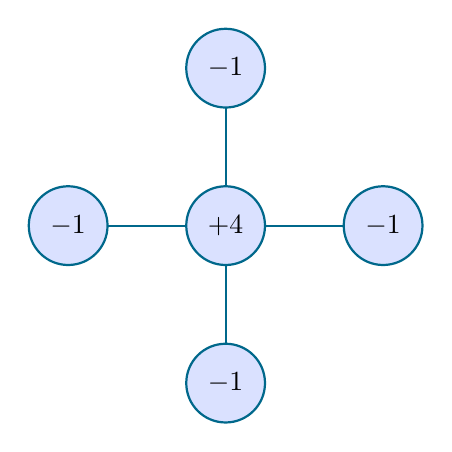
\begin{tikzpicture}[
  every node/.style={
    shape=circle,
    thick,
    fill=cadet,
    draw=darkblue,
    minimum size=1cm,
  }]
  \draw[thick, darkblue] (-2,0) -- (2,0);
  \draw[thick, darkblue] (0,-2) -- (0,2);
  \node at (-2,0) {$-1$};
  \node at (2,0) {$-1$};
  \node at (0,-2) {$-1$};
  \node at (0,2) {$-1$};
  \node at (0,0) {$+4$};
\end{tikzpicture}
}
    \end{center}
  \item This results from a double application of the three-point stencil in two
    directions.
    \begin{center}
      \scalebox{0.5}{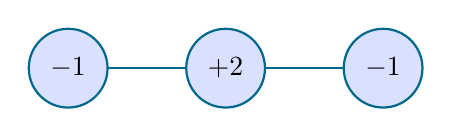
\begin{tikzpicture}[
  every node/.style={
    shape=circle,
    thick,
    fill=cadet,
    draw=darkblue,
    minimum size=1cm,
  }]
  \draw[thick, darkblue] (-2,0) -- (2,0);
  \node at (-2,0) {$-1$};
  \node at (0,0) {$+2$};
  \node at (2,0) {$-1$};
\end{tikzpicture}
}
    \end{center}
  \end{itemize}
\end{frame}

\begin{frame}
  \frametitle{Diagonalization}
  \begin{itemize}
  \item In the following, the matrix $\bm A$ results from the five-point
    stencil (2D problem), while the matrix $\bm T$ results from the three-point
    stencil ($\bm T$).
  \item For a symmetric positive definite matrix $\bm C$, we know that we can
    perform an eigendecomposition
    \[ \bm C \bm Q = \bm Q \bm \Lambda \]
    where $\bm Q$ is the matrix of eigenvectors (as columns) and $\bm \Lambda$
    is the diagonal matrix of eigenvalues.
  \item Since $\bm C$ is SPD, $\bm Q$ is orthogonal, so
    \[ \bm C = \bm Q \bm \Lambda \bm Q^\intercal. \]
  \end{itemize}
\end{frame}

\begin{frame}
  \frametitle{Diagonalization}
  \begin{itemize}
  \item Using this in the linear system, we get
    \[
      \bm C \bm x = \bm b \quad \Longrightarrow \quad
      \bm Q \bm \Lambda \bm Q^\intercal = \bm b.
    \]
  \item Multiply from the left by $\bm Q^\intercal$, recalling that
    $\bm Q^\intercal = \bm Q^{-1}$.
    \[
      \bm \Lambda \underbrace{\bm Q^\intercal \bm x}_{\tilde{\bm x}}
      = \underbrace{\bm Q^\intercal \bm b}_{\tilde{\bm b}}.
    \]
  \item This reduces the problem to three relatively easy steps.
  \end{itemize}
\end{frame}

\begin{frame}
  \frametitle{Diagonalization}
  \begin{enumerate}
  \item Calculate $\tilde{\bm b}$ with a matrix-vector product
    \[ \tilde{\bm b} = \bm Q^\intercal \bm b \]
    in $\mathcal{O}(N^2)$ operations.
  \item Solve the system
    \[ \bm \Lambda \tilde{\bm x} = \tilde{\bm b} \]
    in $\mathcal{O}(N)$ operations ($\bm \Lambda$ is diagonal).
  \item Calculate $\bm x$ with another matrix-vector product
    \[ \bm x = \bm Q \tilde{\bm x} \]
    in $\mathcal{O}(N^2)$ operations.
  \end{enumerate}
\end{frame}

\begin{frame}
  \frametitle{Diagonalization}
  \begin{itemize}
  \item This looks promising: it seems we have found a way to solve the system
    in $\mathcal{O}(N^2)$ operations instead of $\mathcal{O}(N^3)$!
  \item Unfortunately this is not true, as the computation of the
    eigendecomposition itself ($\bm Q$ and $\bm \Lambda$) requires
    $\mathcal{O}(N^3)$ operations.
  \item However, in certain cases we can still exploit this method.
  \end{itemize}
\end{frame}

\begin{frame}
  \frametitle{Diagonalization}
  \begin{itemize}
  \item We constructed the matrix $\bm A$ by applying the three-point stencil in
    two directions.
  \item In the language of linear algebra, this translates to a tensor product.
    \[ \bm A = \bm I \otimes \bm T + \bm T \otimes \bm I \]
  \item The linear system
    \[ \left( \bm I \otimes \bm T + \bm T \otimes \bm I \right) \bm x = \bm b \]
    in a global numbering scheme, can equivalently be stated
    \[ \bm T \bm X + \bm X \bm T^\intercal = \bm B \]
    in a local numbering scheme. Here, the unknown $\bm X$ and the
    right-hand-side $\bm B$ are \emph{matrices}.
  \end{itemize}
\end{frame}

\begin{frame}
  \frametitle{Diagonalization}
  \begin{itemize}
  \item A global numbering scheme is a scheme where we number the unknowns using
    a single index. This naturally maps to a vector.
  \item A local numbering scheme is a scheme where we number the unknowns using
    one index for each spatial direction. This naturally maps to a matrix (in
    2D) or more generally a tensor.
  \item Thus, we consider in this case a system of matrix equations.
  \item Alternative way of thinking about it: we operate with $\bm T$ along the
    columns of $\bm X$, and then along the rows.
    \[
      \underbrace{\bm T \bm X}_{\text{columns}} +
      \underbrace{\left( \bm T \bm X^\intercal \right)^\intercal}_{\text{rows}}
      = \bm T \bm X + \bm X \bm T^\intercal
    \]
  \end{itemize}
\end{frame}

\begin{frame}
  \frametitle{Diagonalization}
  \begin{itemize}
  \item Now let us diagonalize $\bm T$, recalling that it is SPD.
    \begin{align*}
      \bm T \bm X + \bm X \bm T^\intercal &= \bm B \Rightarrow \\
      \bm Q \bm \Lambda \bm Q^\intercal \bm X + \bm X \bm Q \bm \Lambda \bm Q^\intercal &= \bm B.
    \end{align*}
  \item Multiply with $\bm Q$ from the right,
    \[
      \bm Q \bm \Lambda \bm Q^\intercal \bm X \bm Q + \bm X \bm Q \bm \Lambda
      = \bm B \bm Q
    \]
  \item and by $\bm Q^\intercal$ from the left,
    \[
      \bm \Lambda \underbrace{\bm Q^\intercal \bm X \bm Q}_{\tilde{\bm X}} +
      \underbrace{\bm Q^\intercal \bm X \bm Q}_{\tilde{\bm X}} \bm \Lambda =
      \underbrace{\bm Q^\intercal \bm B \bm Q}_{\tilde{\bm B}},
    \]
    or
    \[
      \bm \Lambda \tilde{\bm X} + \tilde{\bm X} \bm \Lambda = \tilde{\bm B}.
    \]
  \end{itemize}
\end{frame}

\begin{frame}
  \frametitle{Diagonalization}
  We find the solution in three steps
  \begin{enumerate}
  \item Calculate $\tilde{\bm B}$ with two matrix-matrix products
    \[ \tilde{\bm B} = \bm Q^\intercal \bm B \bm Q \]
    in $\mathcal{O}(n^3)$ operations.
  \item Solve the system
    \[ \tilde{x}_{i,j} = \frac{\tilde{b}_{i,j}}{\lambda_i + \lambda_j} \]
    in $\mathcal{O}(n^2)$ operations.
  \item Recover the solution with two matrix-matrix products\
    \[ \bm X = \bm Q \tilde{\bm X} \bm Q^\intercal \]
    in $\mathcal{O}(n^3)$ operations.
  \end{enumerate}
\end{frame}

\begin{frame}
  \frametitle{Diagonalization}
  \begin{itemize}
  \item Note that $n = \sqrt{N}$ in two dimensions.
  \item That gives $\mathcal{O}(N^{\nicefrac{3}{2}})$ operations in total, and a
    space complexity of $\mathcal{O}(N)$. A very fast algorithm!
  \item Computing the eigendecomposition is also
    $\mathcal{O}(N^{\nicefrac{3}{2}})$. Since the matrix is smaller, this no
    longer dominates the running time.
  \item It is parallelizable: a few large, global data exchanges are needed
    (transposing matrices). Multiplying matrices can be done with relatively
    little communication. (More on this in the big project.)
  \item LU decomposition would require $\mathcal{O}(N^3)$ operations and
    $\mathcal{O}(N^2)$ storage. Bandewd LU decomposition would require
    $\mathcal{O}(N^2)$ operations and $\mathcal{O}(N^{\nicefrac{3}{2}})$
    storage.
  \end{itemize}
\end{frame}

\begin{frame}
  \frametitle{Diagonalization}
  \begin{itemize}
  \item The diagonalization method is quite general, applicable to any SPD
    system with a tensor-product operator.
  \item We used Poisson to make it more easily understandable (I hope).
  \item It turns out that we can do even better by exploiting even more
    structure in the Poisson problem.
  \end{itemize}
\end{frame}

\begin{frame}
  \frametitle{Diagonalization}
  \begin{itemize}
  \item The continuous eigenvalue problem
    \begin{align*}
      -u_{xx} &= \lambda u, \qquad \text{ in } \Omega = (0,1), \\
      u(0) = u(1) &= 0
    \end{align*}
    has solutions for $j = 1,2,\ldots$
    \begin{align*}
      \overline u_j(x) &= \sin (j\pi x), \\
      \overline \lambda_j &= j^2 \pi^2
    \end{align*}
    \item We now consider operating with $\bm T$ on vectors consisting of $u_j$
      sampled at the gridpoints, i.e.
      \[
        \overline {\bm q}^{(j)}_i = \overline u_j(x_i) = \sin \left( \frac{ij\pi}{n} \right)
      \]
  \end{itemize}
\end{frame}

\begin{frame}
  \frametitle{Diagonalization}
  \begin{itemize}
  \item This yields
    \[
      (\bm T \overline {\bm q}^{(j)})_i =
      \underbrace{2 \left( 1 - \cos \left( \frac{j\pi}{n} \right)
        \right)}_{\lambda_j}
      \underbrace{\sin\left( \frac{ij\pi}{n} \right)}_{\overline {\bm q}^{(j)}_i}
    \]
  \item Thus, the eigenvectors of $\bm T$ are the eigenfunctions of
    $-\nicefrac{\partial^2}{\partial x^2}$ sampled at the gridpoints. (Lucky!)
  \item Let us normalize to obtain the matrix $\bm Q$.
    \begin{align*}
      \bm q_j^\intercal \bm q_j = 1 \Rightarrow
      \bm Q_{i,j} &= \sqrt{\frac{2}{n}} \sin\left( \frac{ij\pi}{n} \right) \\
      \bm \Lambda_{i,i} &= 2\left( 1 - \cos\left( \frac{j\pi}{n} \right) \right)
    \end{align*}
  \end{itemize}
\end{frame}

\begin{frame}
  \frametitle{Discrete Fourier Transform}
  \begin{itemize}
  \item Now for something completely different. (But not really. It's a magic
    trick.)
  \item Consider a periodic function $v(x)$ with period $2\pi$.
  \item Sample this function at equidistant points $x_j$, $j=0,1,\ldots,n$.
  \item As with the finite difference grid, $x_j = jh$ where
    $h = \nicefrac{2\pi}{N}$.
  \item We name the samples $v_j = v(x_j)$.
  \end{itemize}
  \begin{center}
    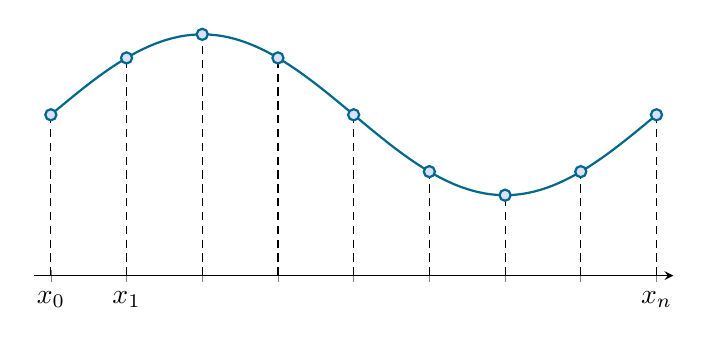
\begin{tikzpicture}
  \begin{axis}[
    width=0.8\textwidth,
    height=0.4\textwidth,
    xmin=-10,
    xmax=370,
    ymin=0,
    ymax=3.2,
    axis lines=middle,
    axis x line=center,
    hide y axis,
    xtick={0.1, 45, 90, 135, 180, 225, 270, 315, 360},
    xticklabels={$x_0$, $x_1$, $$, $$, $$, $$, $$, $$, $x_n$},
    ]
    \addplot[darkblue, thick, domain=0:360, samples=100]{sin(x) + 2};
    \draw[thin, densely dashed] (axis cs:0,0) -- (axis cs:0,2);
    \draw[thin, densely dashed] (axis cs:45,0) -- (axis cs:45,2.707);
    \draw[thin, densely dashed] (axis cs:90,0) -- (axis cs:90,3);
    \draw[thin, densely dashed] (axis cs:135,0) -- (axis cs:135,2.707);
    \draw[thin, densely dashed] (axis cs:180,0) -- (axis cs:180,2);
    \draw[thin, densely dashed] (axis cs:225,0) -- (axis cs:225,1.293);
    \draw[thin, densely dashed] (axis cs:270,0) -- (axis cs:270,1);
    \draw[thin, densely dashed] (axis cs:315,0) -- (axis cs:315,1.293);
    \draw[thin, densely dashed] (axis cs:360,0) -- (axis cs:360,2);
    \node[shape=circle, draw=darkblue, thick, fill=cadet, inner sep=0.5mm] at (axis cs:0,2) {};
    \node[shape=circle, draw=darkblue, thick, fill=cadet, inner sep=0.5mm] at (axis cs:45,2.707) {};
    \node[shape=circle, draw=darkblue, thick, fill=cadet, inner sep=0.5mm] at (axis cs:90,3) {};
    \node[shape=circle, draw=darkblue, thick, fill=cadet, inner sep=0.5mm] at (axis cs:135,2.707) {};
    \node[shape=circle, draw=darkblue, thick, fill=cadet, inner sep=0.5mm] at (axis cs:180,2) {};
    \node[shape=circle, draw=darkblue, thick, fill=cadet, inner sep=0.5mm] at (axis cs:225,1.293) {};
    \node[shape=circle, draw=darkblue, thick, fill=cadet, inner sep=0.5mm] at (axis cs:270,1) {};
    \node[shape=circle, draw=darkblue, thick, fill=cadet, inner sep=0.5mm] at (axis cs:315,1.293) {};
    \node[shape=circle, draw=darkblue, thick, fill=cadet, inner sep=0.5mm] at (axis cs:360,2) {};
  \end{axis}
\end{tikzpicture}

  \end{center}
\end{frame}

\begin{frame}
  \frametitle{Discrete Fourier Transform}
  \begin{itemize}
  \item Consider the vectors $\bm \varphi_k$, where
    \[ (\bm \varphi_k)_j = \text{e}^{\text{i}kx_j}, \]
    where
    \[ \text{e}^{\text{i}kx_j} = \cos(kx_j) + \text{i} \sin(kx_j). \]
  \item These vectors form a basis for the complex $n$-dimensional space
    $\mathbb{C}^{n}$. In particular, they are orthogonal:
    \[
      \bm \varphi_k^\text{H} \bm \varphi_\ell =
      \begin{cases}
        n, & k = \ell, \\
        0, & k \not= \ell,
      \end{cases}
      \qquad k, \ell = 0,1,\ldots,n-1.
    \]
  \end{itemize}
\end{frame}

\begin{frame}
  \frametitle{Discrete Fourier Transform}
  \begin{itemize}
  \item Since they form a basis, any vector in the space can be expressed as a
    linear combination of these vectors.
  \item The vector
    \[
      \bm y = \begin{pmatrix} v_0 & \cdots & v_{n-1} \end{pmatrix}^\intercal \in
      \mathbb{R}^n
    \]
    can be expressed as
    \[
      \bm y = \sum_{k=0}^{n-1} \hat{v}_k \bm \varphi_k,
    \]
    or element by element,
    \[
      v_j = \sum_{k=0}^{n-1} \hat{v}_k (\bm \varphi_k)_j
      = \sum_{k=0}^{n-1} \hat{v}_k \text{e}^{\text{i}kx_j}.
    \]
  \end{itemize}
\end{frame}

\begin{frame}
  \frametitle{Discrete Fourier Transform}
  \begin{itemize}
  \item Here $\hat{v}_k$ are the discrete Fourier coefficients, which are given
    by the inverse relation. (Since $\bm \varphi_k$) are orthogonal, this is
    easy to compute.)
    \[
      \hat{v}_k = \frac{1}{n} \sum_{j=0}^n v_j \text{e}^{\text{i}kx_j}.
    \]
  \item The Fourier transform is extremely useful and has been extensively
    studied.
  \item It is useful in, among other things, signal analysis, audio and video
    compression.
  \item Important property: the DFT coefficients of an odd, real signal are
    purely imaginary.
  \end{itemize}
\end{frame}

\begin{frame}
  \frametitle{Discrete Sine Transform}
  \begin{itemize}
  \item A transform closely related to DFT is the discrete sine transform, the
    DST.
  \item It applies to a function $v(x)$, periodic with period $2\pi$, and
    \emph{odd}. That is, $v(x) = -v(-x)$
  \item We discretize this function on an equidistant mesh between 0 and $\pi$.
    (The values between $\pi$ and $2\pi$ aren't needed because it is odd.)
  \item Since $v$ is odd, we also know that $v(x_0) = v(x_n) = 0$. (These are
    our Poisson boundary conditions.)
  \item Thus the discrete function is represented by the vector
    \[
      \bm y = \begin{pmatrix} v_1 & \cdots & v_{n-1} \end{pmatrix}^\intercal
      \in \mathbb{R}^{n-1}.
    \]
  \end{itemize}
\end{frame}

\begin{frame}
  \frametitle{Discrete Sine Transform}
  \begin{itemize}
  \item As a basis for this space, let us use the sines
    \[
      (\bm \psi_k)_j = \sin\left( \frac{kj\pi}{n} \right),
      \qquad j = 1,\ldots,n-1,
    \]
    and note that
    \[
      \bm \psi_k^\intercal \bm \psi_\ell =
      \begin{cases}
        \nicefrac{n}{2}, & k = \ell, \\
        0, & k \not= \ell.
      \end{cases}
    \]
  \item Thus
    \[
      v_j = \sum_{k=1}^{n-1} \tilde{v}_k \sin \left( \frac{kj\pi}{n} \right)
      = \left( \bm S^{-1} \tilde{\bm y} \right)_j,
    \]
    and
    \[
      \tilde{v}_k = \frac{2}{n} \sum_{j=1}^{n-1} v_j \sin \left( \frac{jk\pi}{n} \right)
      = \left( \bm S \bm y \right)_k
    \]
  \end{itemize}
\end{frame}

\begin{frame}
  \frametitle{Tying it all toghether}
  \begin{itemize}
  \item In particular, we have
    \[
      \bm Q = \sqrt{\frac{n}{2}} \bm S, \qquad
      \bm Q^\intercal = \sqrt{\frac{2}{n}} \bm S^{-1}.
    \]
    Therefore we can compute a matrix-vector product involving $\bm Q$ or
    $\bm Q^\intercal$ by using the DST.
  \item How to compute the DST quickly? Consider a vector
    \[
      \bm y = \begin{pmatrix} v_1 & \cdots & v_{n-1} \end{pmatrix}^\intercal
      \in \mathbb{R}^{n-1}.
    \]
    Construct the odd extended vector
    \[
      \bm w =
      \begin{pmatrix}
        0 & v_1 & \cdots & v_{n-1} & 0 & -v_{n-1} & \cdots & -v_1
      \end{pmatrix}^\intercal
      \in \mathbb{R}^{2n}.
    \]
  \end{itemize}
\end{frame}

\begin{frame}
  \frametitle{Tying it all toghether}
  \begin{itemize}
  \item It turns out that the DST coefficients of $\bm w$ and the DFT
    coefficients of $\bm w$ are related by
    \[
      \tilde{v}_k = 2\text{i}\hat{w}_k, \qquad
      k=1,\ldots,n-1
    \]
  \item Thus, we can find the DST by computing the DFT of the extended vector,
    multiplying the first $n-1$ coefficients (after the constant mode) by
    $2\text{i}$, and throwing away the rest of them.
  \item This is good because there are very fast algorithms for computing the
    DFT: the infamous Fast Fourier Transform (\emph{FFT}).
  \item One FFT is $\mathcal{O}(n \log n)$, so a matrix-matrix product using the
    FFT is $\mathcal{O}(n^2 \log n)$.
  \end{itemize}
\end{frame}

\begin{frame}
  \frametitle{Tying it all together}
  We find the solution in three steps
  \begin{enumerate}
  \item Calculate $\tilde{\bm B}$ with two matrix-matrix products
    \[ \tilde{\bm B}^\intercal = \bm S^{-1} (\bm S \bm B)^\intercal \]
    in $\mathcal{O}(n^2 \log n)$ operations.
  \item Solve the system
    \[ \tilde{x}_{i,j} = \frac{\tilde{b}_{i,j}}{\lambda_i + \lambda_j} \]
    in $\mathcal{O}(n^2)$ operations.
  \item Recover the solution with two matrix-matrix products\
    \[ \bm X = \bm S^{-1} (\bm S \tilde{\bm X}^\intercal)^\intercal \]
    in $\mathcal{O}(n^2 \log n)$ operations.
  \end{enumerate}
\end{frame}

\end{document}

